\documentclass[a4paper,10pt]{article}
\usepackage[utf8]{inputenc}
\usepackage{graphicx}
\usepackage{circuitikz}

%opening
\title{Curva caratteristica del diodo}
\author{Belliardo Federico, Marco Costa}

\begin{document}

\maketitle

\begin{abstract}
In questa esperienza si sono raccolte delle misure di tensione e di corrente relative ad un diodo in diverse condizioni di lavoro, utilizzando due diverse metodologie di misura: 
una automatizzata con Arduino e una manuale effettuata con due tester da laboratorio. I dati ottenuti sono stati \emph{fittati} per ricavare i parametri caratteristici di funzionameno del particolare diodo utilizzato. In particolare si è misurata la resistenza asintotica del diodo per gradi tensioni e si è cercato di individuarne l'origine.
\end{abstract}

\section{Introduzione al diodo}
Il diodo è il primo componente non lineare che si incontra nel corso di laboratorio di fisica. Il suo funzionamento si basa sui fenomeni elettrodinamici che occorrono quando due 
componenti di silicio drogate rispettivamente con boro (p) e con fosforo (n) vengono messe a contatto. Il risultato è che il diodo agisce come un raddrizzatore cioè lascia passare la corrente in un verso mentre la blocca
se collegato nel senso opposto (i diodi sono dotati di polarizzazione). Si diranno in polarizzazione diretta quando la corrente può scorrere e in polarizzazione inversa quando questa è bloccata.
\\
Considerazioni di meccanica statistica permettono di trovare una legge \emph{corrente-tensione} per il diodo (più dettagliata di quella sopra esposta) chiamata \emph{equazione di Shockley} che viene
in genere scritta come segue: 
\begin{equation}
 I = I_0 (e^{\frac{V}{\eta V_t}}-1)
\end{equation}
Dove $I_0$ è la corrente di saturazione inversa, $V_t$ è la tensione di threshold e $\eta$ è un fattore di forma.
Come si può dedurre dall'equazione, prendendo il limite $V \longrightarrow -\infty$, la corrente di saturazione inversa in modulo è quella che attraverserebbe il diodo 
collegandolo con polarità scambiata ad una differenza di potenziale infinita.
La tensione $V_t$ è uguale nel modello di Shockley a $\frac{k_B T}{e}$, alla temperatura ambiente di $300 K$ vale $k_B T = \frac{1}{40}\, eV$ dunque $V_t = 26 \, mV$ come valore numerico.
Il fattore di forma è invece in genere compreso tra 1 e 2.
\\
I diodi presentano una linea argentata in corrispondenza del catodo (come in figura), in seguito è anche riportato il simbolo circuitale del diodo (figure 1), che è una freccia indicante 
la direzione di polarizzazione diretta.

\begin{figure}[!htb]
\begin{center}
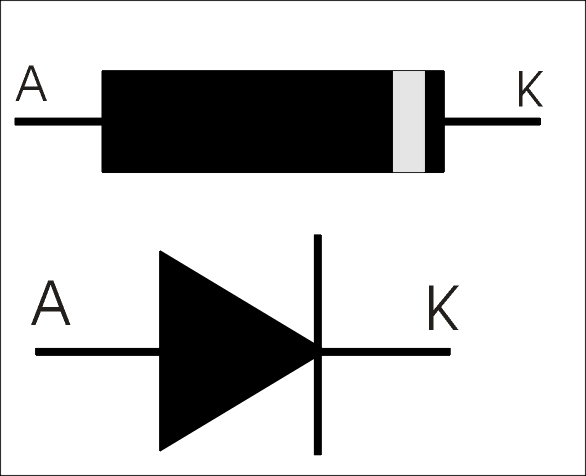
\includegraphics[width=0.3\textwidth]{diodo.jpg}
\end{center}
\caption{Simbolo circuitale del diodo}
\end{figure}

\section{Misure con Arduino}
Per misurare le grandezze che compaiono nella legge di Shockley si è utilizzato un sistema automatizzato di raccolta dati gestito da Arduino. 

\begin{center} \begin{circuitikz}
 \draw  (0,0) to[R, l = $R$] (2,0);
 \draw  (2,0) to[R, l = $R_D$] (4,0);
 \draw	(2,0) to[short, -o, l = $V_1$] (2,2);
 \draw	(4,0) to[short, -o, l = $V_2$] (4,2);
 \draw	(2,0) to[C, l = $C$] (2, -2);
 \draw	(2,-2) to[short] (4, -2);
 \draw	(4, 0) to[diode] (4,-2);
 \draw	(0, -2) to[short] (2, -2);
 \draw	(0,0) to[square voltage source, l= $V(t)$] (0, -2);
 \draw  (0, -2) node[ground] {};
\end{circuitikz} \end{center}

La porta numero cinque di Arduino è stata utilizzata in modalità PWM in modo da produrre un'onda quadra il cui \emph{duty-cycle} era crescente. Il segnale in uscita da Arduino è poi stato inviato ad un integratore costituito da una resistenza di $R=(670\pm5) \, \Omega$ e un condensatore da $C = (220 \pm 50) \, \mu F$: insieme queste componenti costituiscono un circuito integratore avente frequenza di taglio $f = (1.0 \pm 0.2) \, Hz$, dunque  molto minore della frequenza del segnale di Arduino (che è $f = 1 \, kHz$). In questo modo il segnale in uscita dall'integratore è con ottima approssimazione una rampa lineare di potenziale nel tempo.
\\
Le porte analogiche A0 e A2 di Arduino configurate in input sono collegate rispettivamente a V1 e V2. Tutti i potenziali sono misurati rispetto all'uscita GND di Arduino.
\\
Mediante uno script Python che controlla la comunicazione con la porta seriale è possibile anche impostare l'intervallo di tempo tra due acquisizioni successive, che viene di default impostato a $\Delta t = 20 \, ms$. Anche il $duty-cycle$ viene modificato in modo che vada da 0\% a 100\% nel tempo totale in cui viene effettuata la presa dati. Il \emph{duty-cycle} è il tempo che intercorre tra due successivi stati \emph{high} dalla porta scelta di Arduino. La figura 2 è molto esplicativa.

\begin{figure}[!htb]
\begin{center}
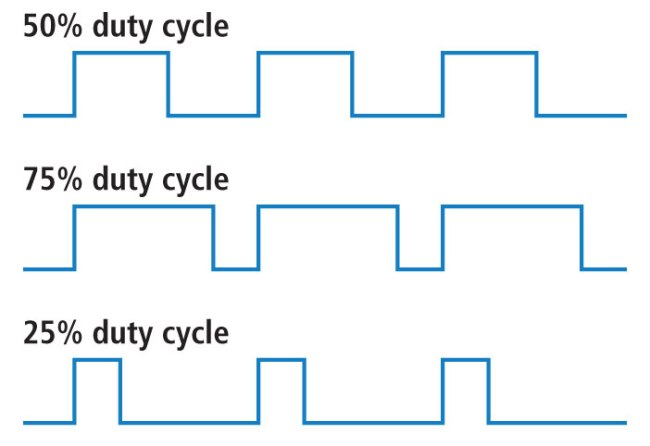
\includegraphics[width=0.5\textwidth]{duty.JPG}
\end{center}
\caption{duty-cycle}
\end{figure}

Il numero delle misure da acquisire è fissato di default a 256. La procedura automatizzata di misura fornisce un file di testo contente i valori letti di V1 e V2 in unità arbitrarie di digitalizzazione, cioè numeri interi da 0 a 1023 (Arduino è dotato di digitalizzatore a 10 bits).
E' dunque necessario misurare $\eta \, (V/digit)$ che è il rapporto di conversione. Per fare ciò si misurerà la differenza di potenziale ($\Delta V$) in uscita dall'integratore, il coefficiente cercato è in tale situazione uguale a $\eta = \frac{\Delta V}{1023}$ cioè $\eta = (4,89 \pm 0,02) \cdot 10^{-3} \; V/digit$.
\\
Si potrebbero eseguire due diverse misure di tensione alla fine del $duty-cycle$: una a diodo collegato e una a diodo scollegato. Esse sono state eseguite e i due risultati sono stati: $V_{collegato} = (4,97\pm0.03) \, V$ e $V_{scollegato} = (5,00\pm0.03) \, V$. I risultati discrepanti sono da attribuire alla resistenza finita del diodo e alla corrente che ci passa attraverso. Le due situazioni sono infatti:

\begin{center}
\textbf{Diodo collegato}
\\
\begin{circuitikz}
\draw (0,0) to[battery1, l = $V_0$] (0,-2);
\draw (0,0) to[R, i>=$i_1$, l = $R_{interna}$]  (2,0);
\draw (2,0) to[generic, i>=$i_3$] (2, -2);
\draw (2,-2) to[short] (0,-2);
\draw (2, 0) to[short, i>=$i_2$] (4, 0);
\draw (4,0) to[voltmeter] (4, -2);
\draw (4, -2) to[short] (2, -2);
\end{circuitikz}
\end{center}

\begin{center}
\textbf{Diodo scollegato}
\\
\begin{circuitikz}
\draw (0,0) to[battery1, l = $V_0$] (0,-2);
\draw (0,0) to[R, i>=$i_4$, l = $R_{interna}$]  (4,0);
\draw (2,-2) to[short] (0,-2);
\draw (4,0) to[voltmeter] (4, -2);
\draw (4, -2) to[short] (2, -2);
\end{circuitikz}
\end{center}
La resistenza $R_{interna}$ è associata alla porta di Arduino scelta.
Nel primo caso, assumendo molto grande la resistenza interna del voltmetro
(sappiamo che R = $10M \Omega $) rispetto alle resistenze $R_{interna}$ e alla resistenza del sistema integratore e diodo, la corrente $i_2$ è piccola, dunque $i_1 \approx i_3$. Quindi il voltmetro misura: $V_{volmetro} = \frac{R_{sistema}}{R_d + R_{sistema}} V_0$, cioè restituisce una misura minore di $V_0$. 
\\
Nel secondo caso, in cui il diodo è scollegato, quando il \emph{duty-cycle} è terminato, il sistema non assorbe corrente: il diodo non c'è e il condensatore è totalmente carico. Dunque la corrente $i_4$ è quella richiesta solamente dal voltmetro, dunque è trascurabile e lo strumento misura esattamente $V_0$

\section{Analisi dei dati - Prima parte}
Dalle misure di $V_1$ e $V_2$ si può calcolare la corrente $I = \frac{V_2 - V_1}{R_d}$ che attraversa il diodo. $V_2$ è poi la differenza di potenziale a cui si trovano i capi del diodo, poiché esso è collegato a terra. Si sono poi propagati gli errori sulla tensione e sulla corrente per ottenere il vettore degli errori $\Delta I$.

\begin{figure}[!htb]
\begin{center}
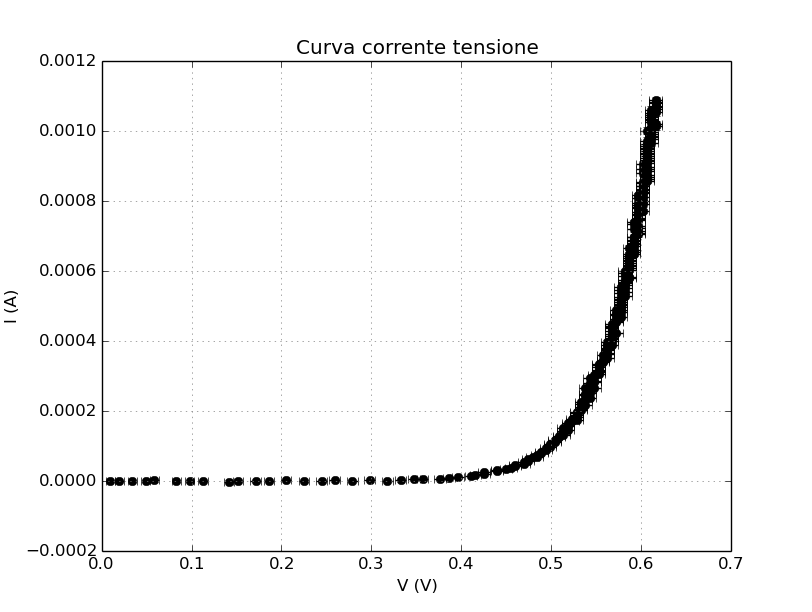
\includegraphics[width=\textwidth]{datiNonFittati.png}
\end{center}
\caption{dati Arduino}
\end{figure}

Il diodo avendo un comportamento non lineare (nella regione di I-V ora esplorata) non ha una resistenza ben definita secondo la legge di Ohm, poiché appunto non è un conduttore Ohmico. E' tuttavia possibile associargli un valore di resistenza dinamica che dipende dalla tensione di lavoro ed è definita come: $R = \frac{dV}{dI}$.

\begin{figure}[!htb]
\begin{center}
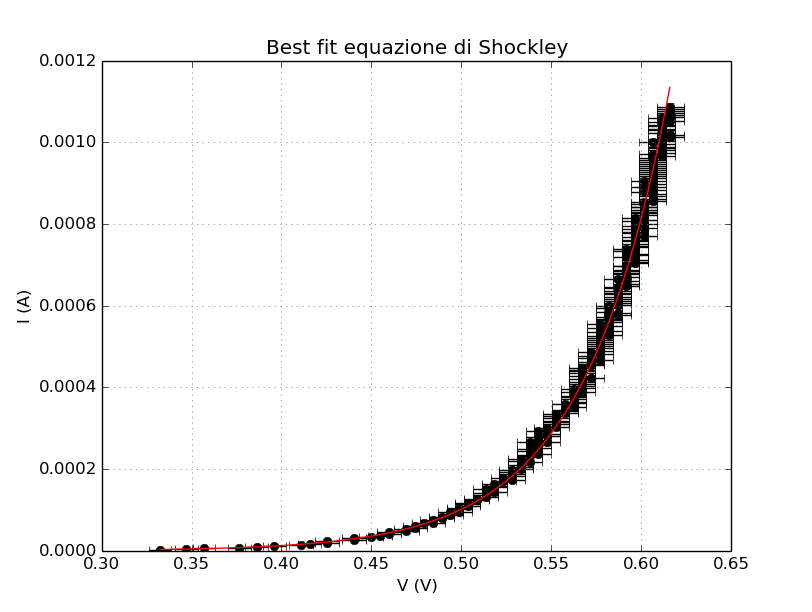
\includegraphics[width=\textwidth]{bestFitShockley.png}
\end{center}
\caption{best-fit}
\end{figure}

Per poter eseguire il \emph{best-fit} (grafico in figura 4) con una legge esponenziale del tipo $I = I_0(e^{\frac{V}{\eta V_t}}+1)$ si sono dovuti eliminare i primi dati raccolti, coi i quali l'algoritmo implementato nelle librerie di \emph{numpy} non riusciva a convergere a un minimo. Ovviamente non è possibile nel \emph{fit} separare la $V_t$ di threshold dal fattore di forma essendo questi completamente correlati.
L'algoritmo di \emph{fit} del minimo $\chi^2$ fornisce i seguenti parametri:
\begin{equation}
\eta V_t = (48,0 \pm 0,1) \cdot 10^{-3}\:V\;\;\;I_0 =(30 \pm 1) \cdot 10^{-10}\:A
\end{equation}
La covarianza normalizzata tra è risultata essere $0,98$ dunque i due parametri del \emph{fit} sono fortemente correlati linearmente, cioè mantenendo costante il $\chi^2$, la variazione di un parametro causa una variazione del secondo che è quasi proporzionale a quella del primo.
\\
Il $\chi^2$ associato a questo \emph{fit} è enorme ($\chi^2 \approx 9000$). Questo è dovuto al fatto che si è scelto di considerare solo l'errore sulle ordinate e al digitalizzatore di Arduino, che associa ad uno stesso voltaggio (discretizzato) una serie di correnti diverse, così che ad ogni voltaggio corrisponde in realtà nel grafico una \emph{"colonna"} di punti. Ciò si può vedere nella figura 5, che è un ingrandimento, in cui sono stati tolti gli errori sui voltaggi per maggior chiarezza.

\begin{figure}[!htb]
\begin{center}
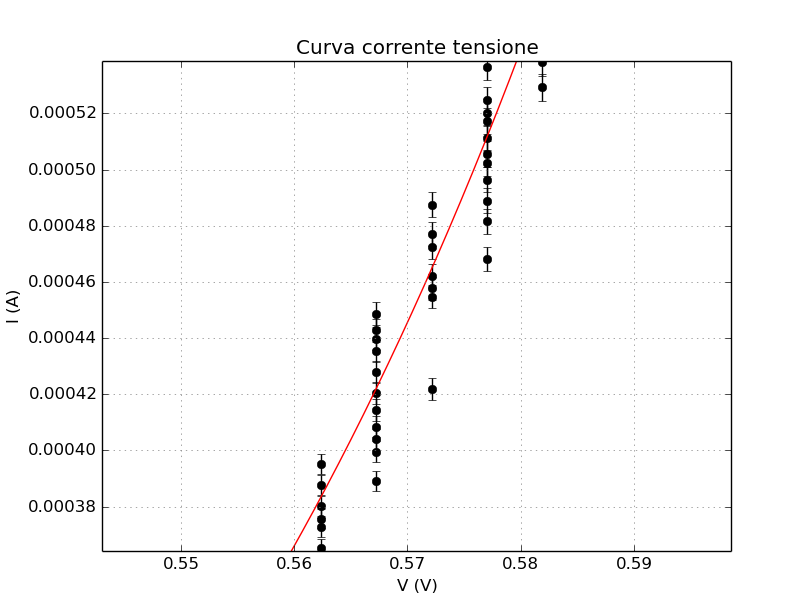
\includegraphics[width=0.8\textwidth]{digitalizzatore.png}
\end{center}
\caption{ingrandimento}
\end{figure}

Per tenere in considerazione nel \emph{fit} anche l'errore sui voltaggi si può scrivere il $\chi^2$ come:
\begin{equation}
\chi^2 = \sum_{i=0}^N \left( \frac{I_i - I(V_i)}{\Delta I_i + \frac{dI}{dV}(V_i) \Delta V_i} \right) ^2
\end{equation}
Dove gli errori si sono sommati come errori strumentali (quindi non in quadratura). 
Questa formula il cui denominatore è stato calcolato propagando l'errore sul numeratore necessita la conoscenza della funzione analitica di \emph{fit}. Essa dunque non può essere utilizzata come primo \emph{best-fit} ma si presta bene ad un procedimento di tipo iterativo.

%Una stima più corretta del chi quadro si può ottenere eseguendo un fit in cui il vettore degli errori 
%$ \Delta I$ è sostituto con un errore costante 
%$ \Delta I = 50 \mu A$, che è circa l'ampiezza di una colonna di punti. E si sostituisce la colonna intera %con un solo punto. DA FARE

Un altro grafico (figura 6) che si può costruire è quello ottenuto invertendo la legge del diodo: $V = \eta V_t log(\frac{I}{I_0} + 1)$, e graficando  il voltaggio in funzione di $log(\frac{I}{I_0} + 1)$. Si dovrebbe ottenere una retta avente coefficiente angolare $\eta V_t$ e intercetta nulla.

\begin{figure}[!htb]
\begin{center}
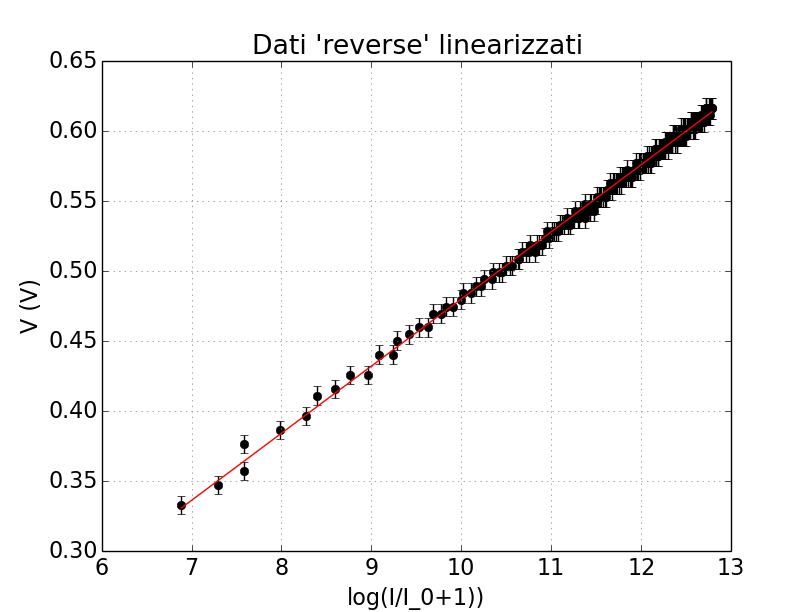
\includegraphics[width=0.8\textwidth]{lin2.png}
\end{center}
\caption{dati linearizzati}
\end{figure}


Il \emph{fit} è stato eseguito con una funzione lineare del tipo $y = ax+b$, questa volta gli unici errori che sono stati tenuti in considerazione sono stati quelli sui voltaggi che sono le ordinate del grafico in figura 6. Nuovamente si potrebbe scrivere un $\chi^2$ che tenga in considerazione anche l'errore sulle correnti, formalmente identico a quello descritto precedentemente (con la semplificazione che la derivata di una funzione lineare è una costante).
I valori ottenuti dal \emph{fit} sono i seguenti:

\begin{equation}
\eta V_t = (48,0 \pm 0,2) \cdot 10^{-3}\:V\;\;\;b =(0 \pm 2) \cdot 10^{-3}\:V
\end{equation}

Dunque il primo parametro $\eta V_t$ è in perfetto accordo con quello ottenuto dal \emph{fit} esponenziale. Si potrebbe fare un test del chi quadro ad un grado di libertà sulla differenza tra i due valori di questo parametro ottenuti dai due \emph{fit} differenti. Il secondo parametro è compatibile con 0, come ci si aspetta nel caso in cui la legge di Shockley sia valida. 

La curva linearizzata mostrata (figura 6) non evidenzia alcuna possibile deviazione dalla legge di Shockley, infatti per trovare un comportamento non lineare bisogna spingersi a tensioni di lavoro molto più elevate.

\section{Misure ad alte tensioni}

Per fare ciò, si è utilizzato un generatore di tensione con un range di lavoro $0-30 \, V$ collegato in serie al diodo ed ad una resistenza. Per eseguire le misure si sono utilizzate due diverse resistenze, una da $R=330 \, \Omega$ in ceramica per i primi sette punti del grafico e in seguito una resistenza a filo da $R = 47 \pm 1 \, \Omega$. Si è inserito un resistore di questo tipo perché le alte correnti ($0,20 - 0,40 \, A$) che passano attraverso il circuito avrebbero bruciato per effetto Joule un qualunque altro tipo di resistenza. Il valore scelto è tale da realizzare un partitore di tensione, che permette di ottenere le differenze di potenziale volute ai capi del diodo.

\begin{center}
\begin{circuitikz}
\draw (0,0) to[R, l=$R$] (2,0);
\draw (2, 0) to[diode, l=$Diodo$] (2, -2);
\draw (0, -2) to[ammeter] (2,-2);
\draw (0, -2) to[battery1, l=$V_0$] (0,0);
\end{circuitikz}
\end{center}

\section{Analisi dati - Seconda parte}

In seguito (figura 7) si riportano i dati corrente tensione ottenuti, sono riportati anche i dati presi con Arduino per confronto (riportate con punti di colore rosso). Si vede infatti che le correnti misurate in questa seconda parte dell'esperienza sono di tre ordini di grandezza superiori a quelle misurate prima.

\begin{figure}[!htb]
\begin{center}
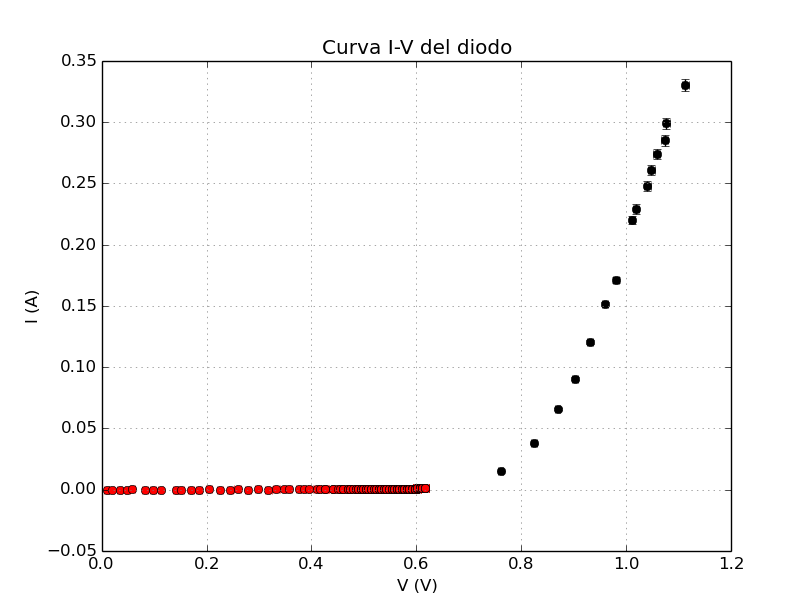
\includegraphics[width=0.9\textwidth]{curvaiv_1.png}
\end{center}
\caption{dati estesi}
\end{figure}

Successivamente sono state prese misure di tensione e corrente per il diodo collegato in modalità reverse. Il \emph{plot} tensione-corrente di tutti i dati ottenuti nell'esperienza è riportato in figura 8.

\begin{figure}[!htb]
\begin{center}
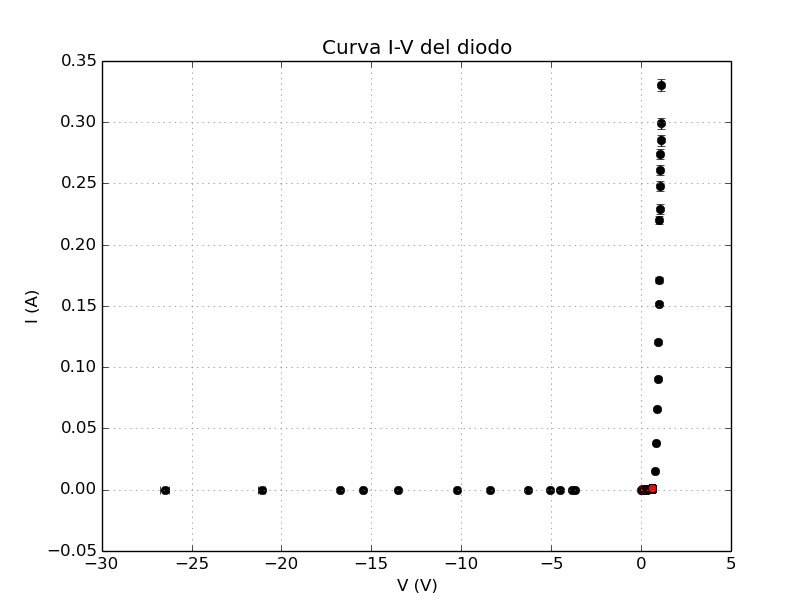
\includegraphics[width=0.9\textwidth]{curvaiv_2.png}
\end{center}
\caption{dati estesi}
\end{figure}

L'accumulo dei punti intorno all'origine colorati di rosso sono i dati presi con Arduino: in questa scala di tensioni e amperaggi non è possibile distinguere il comportamento esponenziale del diodo. Come si vede la funzione corrente-tensione è molto simile ad una funzione a gradino, con altezza "infinita". Questo giustifica l'affermazione fatta nell'introduzione che un diodo lascia passare la corrente in un verso mentre la blocca in senso opposto.

E' poi possibile graficare i nuovi dati (di corrente diretta) su una scala logaritmica come quella usata precedentemente per eseguire il \emph{fit} lineare ottenendo il \emph{plot} in figura 9.
\\
\begin{figure}[!htb]
\begin{center}
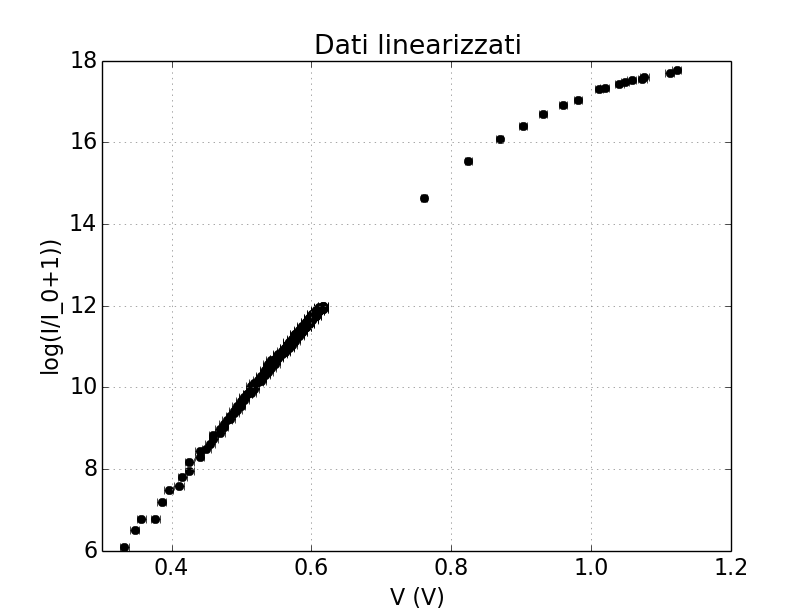
\includegraphics[width=0.8\textwidth]{lin1.png}
\end{center}
\caption{dati linearizzati}
\end{figure}
\\

\section{Resistenza di contatto}
Come si vede dal grafico precedente per grandi voltaggi ho una deviazione dalla legge di Shockley, infatti il comportamento asintotico del diodo è lineare: questo è dovuto al prevalere della componente ohmica del diodo sugli effetti dalla giunzione p-n vera e propria.

Con una regressione lineare è possibile stimare la resistenza asintotica del diodo (figura 10).

\begin{figure}[!htb]
\begin{center}
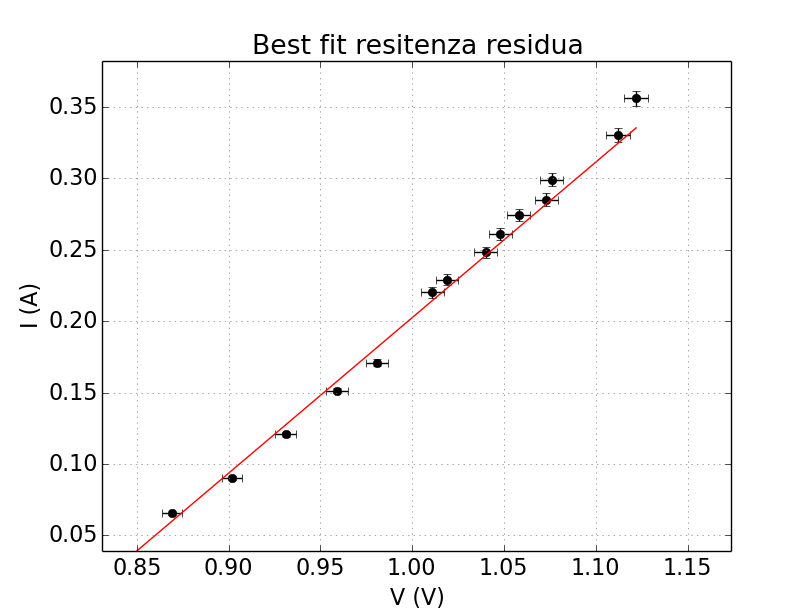
\includegraphics[width=0.8\textwidth]{resistenzaResidua.png}
\end{center}
\caption{resistenza asintotica}
\end{figure}

I parametri che si ottengono dal \emph{fit} sono:
\begin{equation}
R = (0,92 \pm 0,03) \, \Omega \;\;\; I_0=(-0,87 \pm 003) \, A
\end{equation}
Il $\chi^2 = 5 \;\; l = 12$ ottenuto indica che consistentemente con gli errori di misura strumentali utilizzati i dati sono ben approssimati da una retta.
Inoltre la covarianza normalizzata risulta essere: 0.029, dunque i due parametri sono poco correlati. L'intercetta è poco importante in realtà in quanto non ha significato fisico. Mentre vediamo che il coefficiente angolare indica che il diodo ha una resistenza ohmica residua di circa $1 \, \Omega$.
Questa è la resistenza dinamica asintotica del diodo nel senso che è l'inverso del coefficiente angolare della curva I-V in punti in cui la tensione è maggiore di $0,7\,V$ che è circa il valore di tensione a cui si trova il "gomito" nel grafico in figura 7. Questo valore di tensione discrimina due regioni di operazione del diodo in cui esso si comporta rispettivamente da diodo ideale e da resistenza ohmica.
\\
Questa resistenza residua è dovuta alla presenza dei contatti ohmici ai lati della giunzione di silicio. Con il termine contatto ohmico ci i riferisce alla regione di collegamenti tra i conduttori che costituiscono anodo e catodo del diodo e il semiconduttore. La fabbricazione di contatti che seguano la legge di Ohm, presentino piccole resistenze e siano stabili è uno dei problemi più importanti dell'ingegneria dei materiali.
\\
In particolare la presenza di una capacità associata al contatto determina la comparsa di una costante di tempo \emph{RC} che limita la risposta del dispositivo ad alte frequenze. Inoltre nell'elettronica la resistenza dei contatti è la causa principale di dissipazione di energia per effetto Joule. Uno dei più importanti problemi dell'ingegneria dei semiconduttori è quindi la realizzazione di contatti efficienti. Nei diodi al silicio i materiali più usati per realizzare il contatto ohmico sono: $Al, Al-Si, TiSi_2, TiN, W, MoSi_2, PtSi, CoSi_2, WSi_2$.
\\
La giunzione metallo semiconduttore presenta anche una componente capacitiva, di difficile misurazione, dunque uno schema possibile per un diodo reale è riportato in basso dove si sono modellati i contatti come resistenze aventi in parallelo una capacità (questa non può essere in serie al diodo perché sappiamo che a regime il componente lascia passare corrente, cosa che non farebbe un condensatore). 
Questa ipotesi non verrà quindi analizzata in seguito.

\begin{center}
\begin{circuitikz}
\draw (0,0) to[short] (2,0);
\draw (2,0) to[short] (2,2);
\draw (2,2) to[C, l=$C$] (4,2);
\draw (4,2) to[short] (4,0);
\draw (2,0) to[R, l=$R$] (4,0);
\draw (4, 0) to[diode, l=$Diode$] (6, 0);
\draw (6,0) to[R, l=$R$] (8,0);
\draw (6,0) to[short] (6,2);
\draw (6,2) to[C, l=$C$] (8,2);
\draw (8,2) to[short] (8,0);
\draw (8,0) to[short] (10,0);
\draw (0,0) to[short] (0, -2);
\draw (0,-2) to[battery1, l=$V_0$] (10, -2);
\draw (10,-2) to[short] (10,0);
\end{circuitikz}
\end{center}

\end{document}
